\documentclass[a4paper, 12pt]{report}

%%%%%%%%%%%%
% Packages %
%%%%%%%%%%%%

\usepackage[english]{babel}
\usepackage[noheader]{packages/sleek}
\usepackage{packages/sleek-title}
\usepackage{packages/sleek-theorems}
\usepackage{packages/sleek-listings}

\usepackage{fontspec}
\usepackage[CheckSingle, CJKmath]{xeCJK}
\usepackage{CJKulem}

\setCJKmainfont{Noto Sans CJK TC}

%%%%%%%%%%%%%%
% Title-page %
%%%%%%%%%%%%%%

\logo{./resources/pdf/blank.png}
\institute{輔仁大學資訊工程學系}
\faculty{畢業專題報告}
\department{B03 組}
\title{Rish Engine - 2D 遊戲引擎}
\subtitle{從零開始自幹遊戲引擎}
\author{\textit{成員} \\
	406262515 \textsc{鍾秉桓} me@roy4801.tw\ \ \ \ \ \ \ \ \ \ \ \ \ \ \\
    406262084 \textsc{梁博全} me@icejj.tw\ \ \ \ \ \ \ \ \ \ \ \ \ \ \ \ \ \ \  \\
    406262319 \textsc{黃育晧} suntalk1224@gmail.com\ \  \\
    406262163 \textsc{黃品翰} william31212@gmail.com \\
    \ \\
    報告編號: CS109-PR-B03 \\
    \ \\
    \textit{指導教授} \\
    鄭進和
}
%\supervisor{Linus \textsc{Torvalds}}
%\context{Well, I was bored...}
\date{\today}

%%%%%%%%%%%%%%%%
% Bibliography %
%%%%%%%%%%%%%%%%

\addbibresource{./resources/bib/references.bib}

%%%%%%%%%%
% Others %
%%%%%%%%%%

\lstdefinestyle{latex}{
    language=TeX,
    style=default,
    %%%%%
    commentstyle=\ForestGreen,
    keywordstyle=\TrueBlue,
    stringstyle=\VeronicaPurple,
    emphstyle=\TrueBlue,
    %%%%%
    emph={LaTeX, usepackage, textit, textbf, textsc}
}

\FrameTBStyle{latex}

\def\tbs{\textbackslash}

%%%%%%%%%%%%
% Document %
%%%%%%%%%%%%

\begin{document}
    \maketitle
    \romantableofcontents

    \chapter{摘要}

\section{背景簡介}

本專題是以 C++ 開發之 2D 遊戲引擎,開發者可以使用引擎提供之編輯器(RishEditor)編輯遊戲場景(Scene),並且可以對遊戲物件(Entity)附加遊戲邏輯(使用C++撰寫,並和編輯器一同編譯),
並支援 Batch Rendering \footnote{一種 Rendering 技巧,可支援同屏幕高達 100000 個 sprites} 、2D Lighting (Point Light, Ambient Light), Particle System, Constrain-based Physics (支援圓形、多邊形等)

\section{問題說明}

TODO

\section{實作結果}

TODO 本專題製作解決問題方法、創新所在、與實作結果等概要陳述

\newpage
    \chapter{緒論}

\section{動機}

隨著遊戲的發展,現代的遊戲越來越趨於複雜,從數人的小型獨立製作,到數百人的大型 3A 級遊戲,遊戲的規模與以前不可同日而語,現今一個獨立開發工作室製作的 2D 遊戲,
在十多年前要達到同樣的規模可能要數十人的團隊才可能達到,而這些節省下來的時間成本,就是多虧了遊戲引擎的強大之處。現代遊戲引擎的複雜度,先進的圖學技術,複雜的物理模擬,
是需要一個具有規模的團隊來開發的,我們嘗試以此為目標,試著實作了一個具有一定規模的 2D 遊戲引擎。

\section{問題描述}

\subsection{歷史介紹}

最初並沒有所謂的遊戲引擎,遊戲常常是重頭開始建構(from scratch)的,這個概念被眾人所知最早是由 Jhon Carmack 發揚光大,他為 Doom 以及 Quake 系列遊戲開發的 3D 遊戲引擎,
深深地影響了遊戲業界,為早期(1990末)的遊戲業界標準,並促成引擎授權的商業模式,使得遊戲軟體的規模上升。

\subsection{遊戲是什麼}
電腦遊戲的技術本質是實時(real-time)可交互(interactive)的程式,遊戲程式會模擬出不精確但足以表現的遊戲世界,並且根據玩家的輸入做出相對的輸出(例如操作搖桿控制角色等),
通常遊戲會實作遊戲循環(Game Loop),更新遊戲邏輯、物理模擬、更新 AI 等。而通常遊戲要維持在每秒更新 60 幀才能保證流暢運行(低於 60 fps 通常會感覺卡頓),
也就是要在 16 毫秒內做完所有的遊戲更新並渲染到螢幕上頭,更何況在 VR 上要維持 90 FPS 才不會感覺暈眩,這也是為甚麼遊戲會如此要求效能。

\subsection{遊戲引擎是什麼}

遊戲引擎(Game Enigne)從字面上解釋是驅動遊戲的基礎程式,因此遊戲引擎須具備了窗口管理、輸出入管理、渲染(Rendering)系統、物理(Physics)系統…等子系統,除了基礎程式之外,
要是一個遊戲引擎還必須要有讓遊戲開發者使用之工具(可視化、非可視化),可能是單個工具或一整個工具鏈(Toolchain),使得遊戲開發者可以用該工具開發遊戲(Developing)、
進行測試(Debugging)、封裝發布(Shipping)等,否則就只能被稱為遊戲框架(Game Framework)。
遊戲引擎會讀入自訂的資源(Asset)格式 \footnote{常常是為了效能才會這樣做},並且有工具支援設計師將素材(貼圖、音效、模型等)轉換成引擎的格式,或是引擎工具可以直接產生,
因此遊戲引擎可以說是專門開發遊戲的開發環境。

\subsection{遊戲引擎具備的功能}

TODO

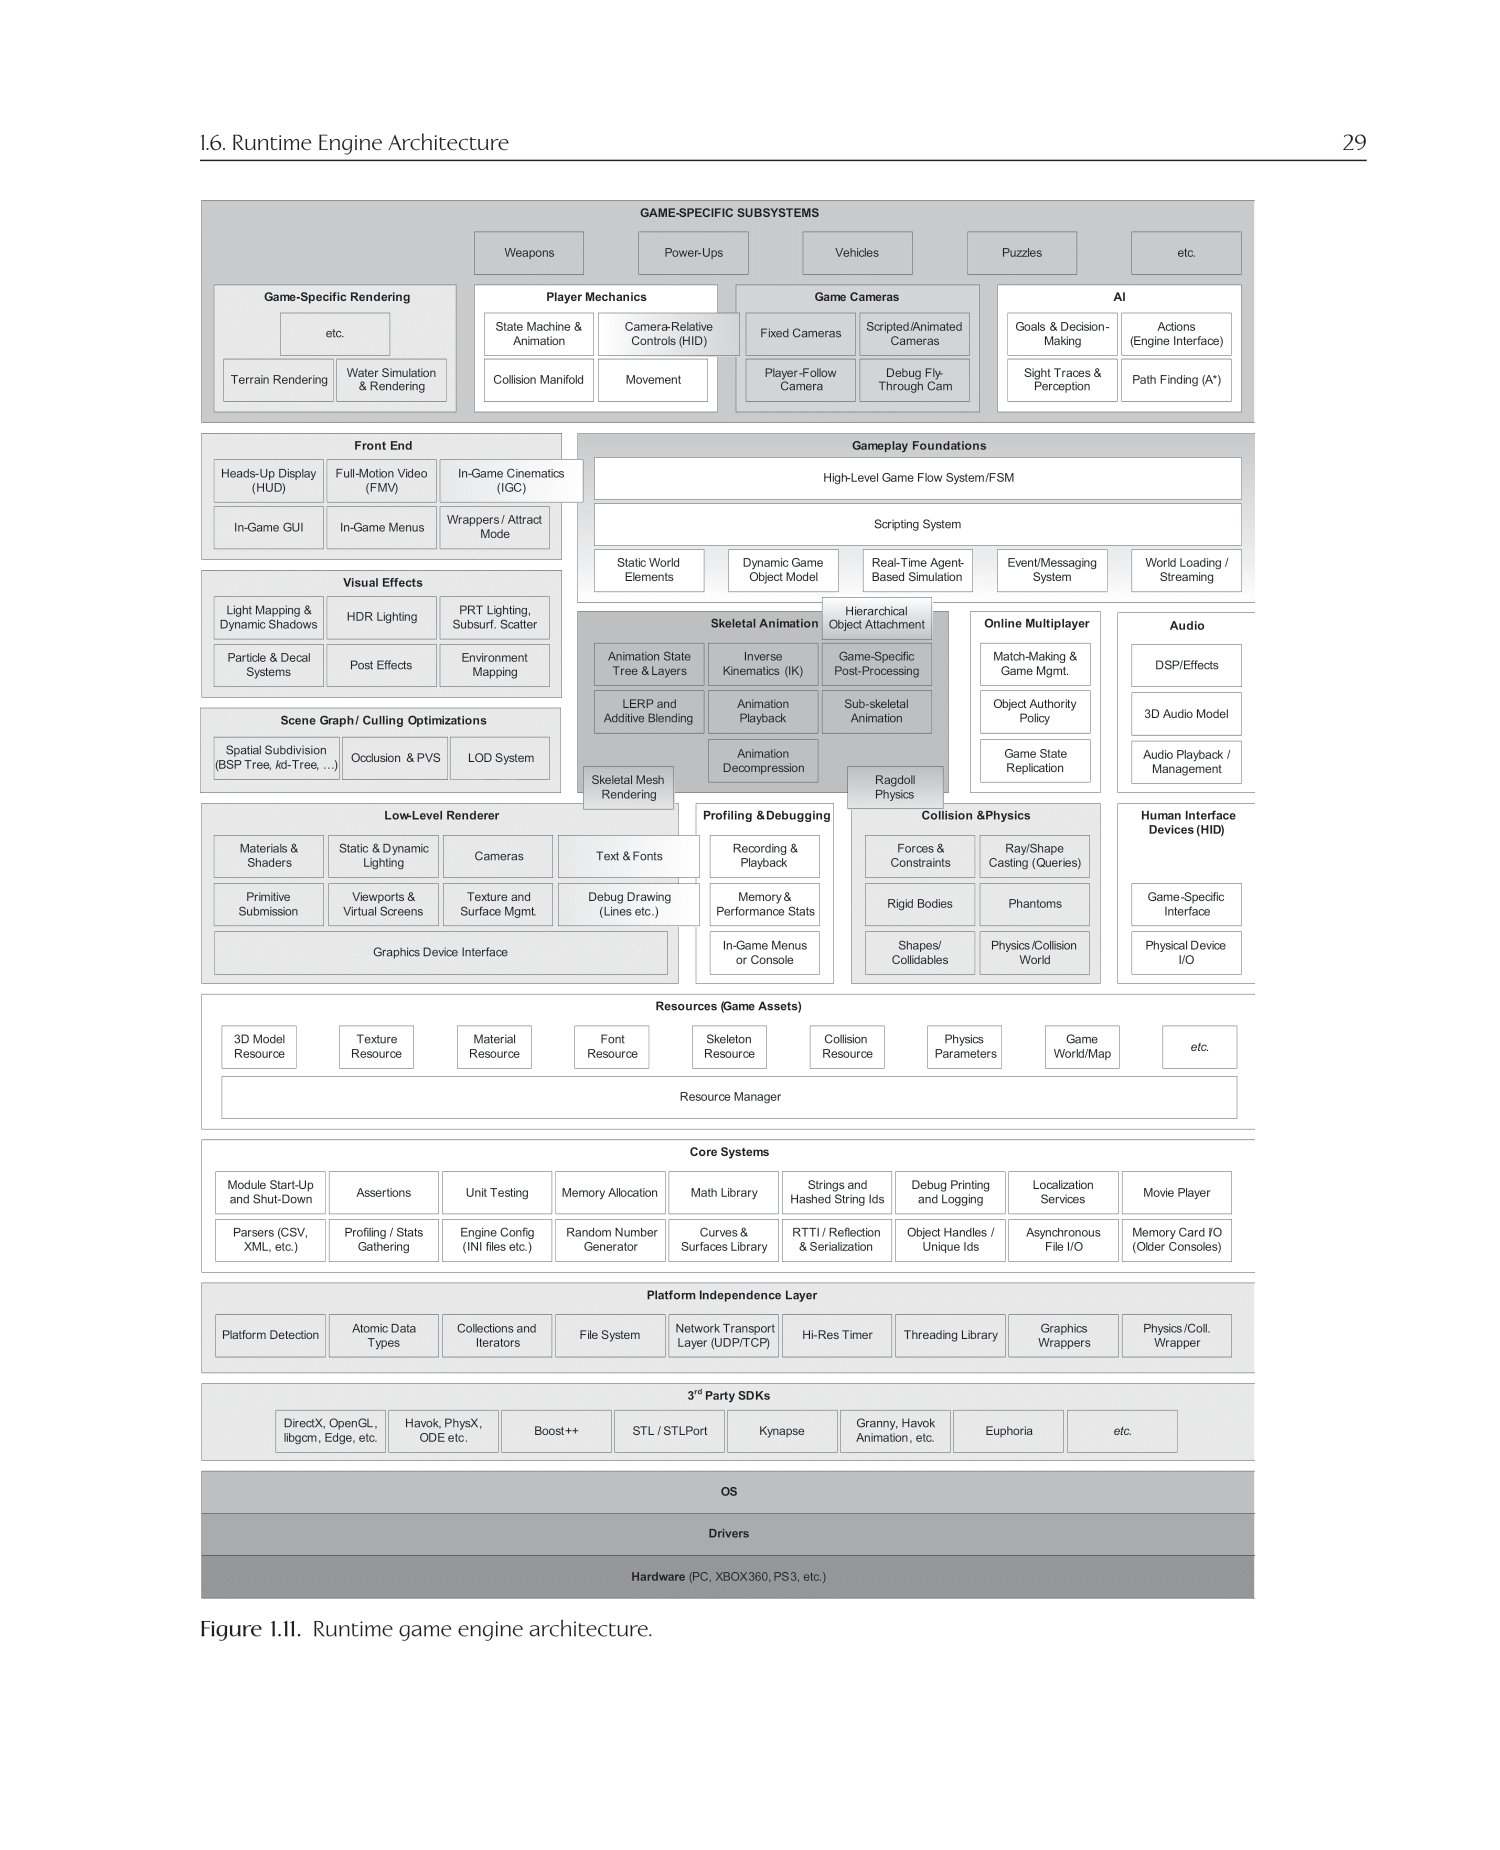
\includegraphics[width=\textwidth]{./resources/engine_arch.png}

\newpage
    \chapter{系統說明}

\section{使用技術}

\subsection{使用語言}

使用 C++ 11 作為主要開發語言,使用 msys2 作為套件管理器 \footnote{在 Windows 上,沒有套件管理器會非常痛苦} ,CMake 建置專案,
使用 doxygen 工具將註解轉換 documentation, cppcheck C++ 的靜態程式碼分析器

\begin{itemize}
	\item{Slack}
		\subitem{團隊協作軟體,用於溝通紀錄}
	\item{Trello}
		\subitem{看板軟體,用於工作進度管理}
	\item{git, github}
		\subitem{版本控制}
\end{itemize}

TODO 寫多一點

\subsubsection{為何選 C++ 做為開發引擎之語言?}

因為 C++ 讓開發者可以自由掌控記憶體,讓開發者可以精確的控制變數的生命週期,沒有垃圾回收(Garbage Collection),這對於效能注重的遊戲引擎來說相當重要;
比 C 來得高階但效能卻沒損失很多;C++ 歷史悠久且有許多精良的函式庫可以使用。 \cite{WhyCppUsedInGameEngine}

\subsubsection{使用函式庫}

\begin{itemize}
	\item{\href{https://www.sfml-dev.org/}{SFML}}
		\subitem{一個 C++ 的跨平台用於遊戲、多媒體程式開發的函式庫,於此專案中用於 Input 及窗口操作等}

	\item{OpenGL + \href{https://github.com/Dav1dde/glad}{glad}}
		\subitem{一個跨平台的 API ,使用 glad 載入器}

	\item{\href{https://github.com/ocornut/imgui}{imgui}}
		\subitem{一個輕量、快速的 Immediate Mode GUI 函式庫,常在遊戲開發、工具開發等使用,於此專案中用於編輯器的 UI 開發。}

	\item{\href{https://github.com/gabime/spdlog}{spdlog}}
		\subitem{一個輕量、快速的 Logging 函式庫,於此專案中用於處理除錯訊息。}

	\item{\href{https://github.com/mlabbe/nativefiledialog}{nativefiledialog}}
		\subitem{小型的 Open File Dialog 函式庫,於此專案中用於處理開啟檔案視窗。}

	\item{\href{https://github.com/juliettef/IconFontCppHeaders}{IconFontCppHeaders}}
		\subitem{字體的 Helper Headers,於此專案中用於引入自訂字體。}

	\item{\href{https://github.com/fmtlib/fmt}{fmt}}
		\subitem{補足了 C++ 標準庫缺少的格式化輸出輸入。}

	\item{\href{https://github.com/g-truc/glm}{glm}}
		\subitem{OpenGL 數學函式庫,於此專案中用於處理向量、投影等相關數學函式。}

	\item{\href{https://github.com/USCiLab/cereal}{cereal}}
		\subitem{C++ 缺少的序列化函式庫,於此專案中用於序列化儲存資源。}

	\item{\href{https://github.com/google/re2}{re2}}
		\subitem{來自 Google 的 Regular Expression 函式庫,標準庫的有夠慢(確信。}

	\item{\href{}{}}
		\subitem{}
 \end{itemize}

    \chapter{系統實作結果}

\section{引擎介紹}

\subsection{架構}
\label{sub:架構}

\subsubsection{流程圖} % (fold)
\label{ssub:流程圖}



\subsubsection{架構圖} % (fold)
\label{ssub:架構圖}

RishEngine 是由眾多模塊組合而成,就像一個大工具包一樣,給遊戲開發者提供了許多功能:

\begin{itemize}
\item{Core}
    \SubItem{核心模塊,提供了許多基礎功能,例如:檔案系統、視窗、事件、輸出入等功能}
\item{Scene}
    \SubItem{場景模塊,提供了 ECS 和一些跟遊戲物件管理的功能}
\item{Layer}
    \SubItem{提供引擎像是圖層一樣操控遊戲畫面、UI}
\item{Renderer}
    \SubItem{渲染模塊,渲染的基礎建設}
\item{Physics}
    \SubItem{物理引擎,讓東西能動起來}
\item{Particle}
    \SubItem{粒子效果}
\item{Editor}
    \SubItem{編輯器,提供了讓遊戲開發者編輯的工具}
\end{itemize}

\begin{figure}[h]
    \begin{center}
    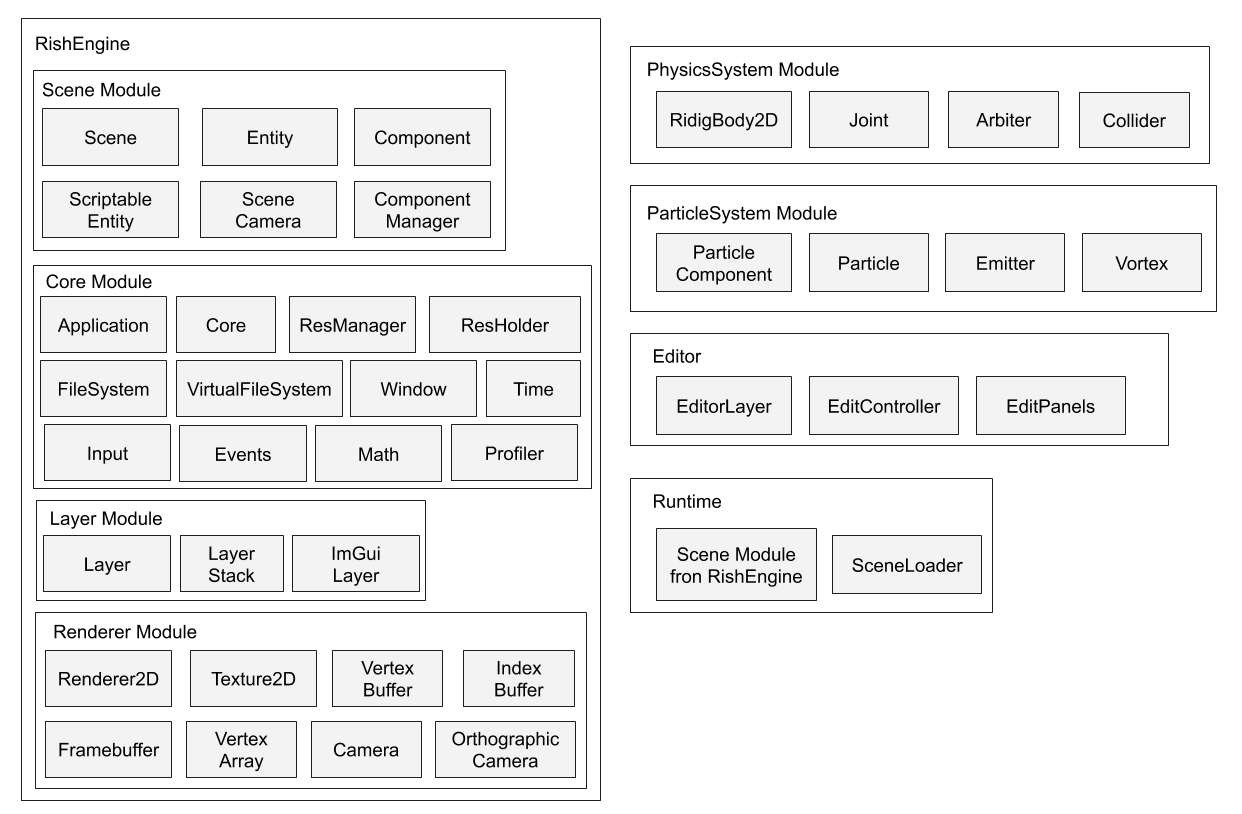
\includegraphics[width=\textwidth]{./resources/RishEngine_arch.png}
    \end{center}
\caption{RishEngine 架構}
\label{fig:RishEngineArch}
\end{figure}


%  Engine
\import{ch4/}{ecs.tex}
\import{ch4/}{batch_rendering.tex}
\import{ch4/}{particle_system.tex}
\import{ch4/}{2d_lighting.tex}
\import{ch4/}{scriptable_entity.tex}
\import{ch4/}{physics.tex}

% Editor
\import{ch4/}{editor.tex}

\newpage
    \chapter{結論與未來展望}

\newpage
    \chapter{心得}

\paragraph{Roy} % (fold)
\label{par:Roy}


其實從高中初次接觸程式設計以來,我一直想做的事情便是寫一個自己的遊戲引擎,從高中時初次嘗試撰寫 ADV 類型的遊戲引擎(但受限當時的程式能力,並沒有完成),而到了大學時,我從很早(大概大二)便找好組員,並且也在系上課程的多個專案中不斷地練習和磨合我們之間的合作,我想做的事便是寫一個屬於自己的遊戲引擎。

從三年級下學期開始,經過了九個月的的開發,坐在電腦前數百小時的奮鬥,我們 RISH 終於將 RishEngine 的功能告一個段落,儘管有些功能是因為專案時程以及目前能力而有缺憾,但即便如此我們還是完成了這個專案,我們開發了一款 2D 的遊戲引擎,具有 ECS、有引擎編輯器、有 Batch Rendering、有 2D Lighting、有物理引擎、有 Particle System 等。

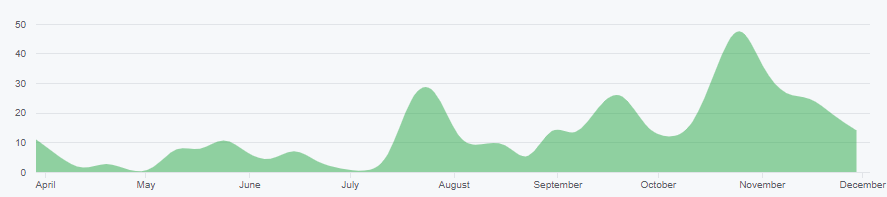
\includegraphics[width=\textwidth]{./resources/commit.png}

而在開發每項功能前,都花了一到兩個星期在做資料搜尋、自學,接著做出最小可行的 Demo,僅僅做出功能還不夠,因為我們做得是遊戲引擎,所以還得將 API 打磨,不斷得去想、擴充功能,因為引擎就是得提供許多功能給遊戲開發者,而在引擎開發階段時,每個功能寫出來之後,還得切換身分到遊戲開發者,試圖用自己做出的引擎來打造遊戲,透過這個過程來除錯和發想可以增加的新功能,一直不斷的迭代,而這個過程是相當漫長和痛苦的,常常在和組員討論時一個功能的規格(spec)時,往往最後都覺得很迷惘,總是覺得這個功能不夠好,但還是得在現實與理想中取捨。

在這次的專案中我也學到了很多東西,像是如何有效與人溝通和合作,表達自己的想法給對方清楚理解,當然過程中勢必有磨合的時期,因為我們是只有四個人的小組,所以作為組長的我理所當然會處理許多工作,也必須擔當起管理的責任,畢竟繁雜的工作量由一個人扛起也過於不切實際,清楚了解到除了程式之外管理和與人相處溝通之道也相當重要。

這個畢業專題算是完成了我其中的一個心願,自幹一個遊戲引擎,也是我目前處理過最多行的程式,算是我的一個小小的里程碑。

% paragraph Roy (end)

\newpage

    \printbibliography


    % \chapter{Introduction}

    Sleek Template is a minimal collection of \LaTeX{} packages and settings that ease the writing of beautiful documents. While originally meant for theses, it is perfectly suitable for project reports, articles, syntheses, etc. -- with a few adjustments, like margins.

    It is composed of four separate packages -- \texttt{sleek}, \texttt{sleek-title}, \texttt{sleek-theorems} and \texttt{sleek-listings} -- each of which can be used individually.

    \begin{lstlisting}[style=latexFrameTB, caption={Example of Sleek Template packages usage.}, gobble=8]
        \usepackage[english]{babel}
        \usepackage[noheader]{packages/sleek}
        \usepackage{packages/sleek-title}
    \end{lstlisting}

    \blindfootnote{If you are a \LaTeX{} beginner consider the excellent \href{https://www.overleaf.com/learn}{Overleaf tutorial}. Also, there are a lot of symbols available in \LaTeX{} and, therefore, in this template. I recommend the use of \enquote{The Comprehensive \LaTeX{} Symbol List} \cite{pakin2020comprehensive} for searching symbols.}

    \chapter{Features}

    \section{\texttt{sleek}}

    \texttt{sleek} is the main package. It imports the packages (\emph{cf.} Table \ref{tab:sleek_relevant_packages}) and setups the settings that make Sleek Template easy to use.

    There are three available options to the \texttt{sleek} package :

    \begin{enumerate}[noitemsep]
        \item \texttt{parindent} add indentation to the first line of paragraphs;
        \item \texttt{noheader} removes the document header;
        \item \texttt{french} changes the decimal sign to a comma and translates some captions.
    \end{enumerate}

    But nothing prevents you to tweak the settings to your liking in the source code.

    \subsection{Mathematics}

    This template uses \texttt{amsmath} and \texttt{amssymb}, which are the de-facto standard for typesetting mathematics. Additionally, \texttt{esint} provides alternative integral symbols (\emph{cf.} Table 78 in \cite{pakin2020comprehensive}) and \texttt{bm} is used for bold math symbols like vectors (see \eqref{eq:gauss_law}).

    A few custom macros have also been added such as \texttt{\tbs{}rbk}, \texttt{\tbs{}sbk} and \texttt{\tbs{}cbk} for respectively round, square and curly brackets, \texttt{\tbs{}abs} for absulute value, \texttt{\tbs{}norm} for norm, \texttt{\tbs{}fact} for factorial and \texttt{\tbs{}diff} for up-right differential.
    $$
        \rbk{\frac{\pi}{2}}, \quad \sbk{\frac{\pi}{2}}, \quad \cbk{\frac{\pi}{2}}, \quad \abs{\frac{\pi}{2}}, \quad \norm{\frac{\pi}{2}}, \quad \fact{n} = \prod_{i = 1}^{n} i, \quad \frac{\diff \bm{x}}{\diff t} = \bm{v}
    $$

    Here are some examples showcasing what is possible with the default packages of \texttt{sleek}.

    \begin{equation}\label{eq:gauss_law}
        \oiint_S \bm{E} \cdot \diff \bm{s} = \iiint_V \frac{\rho}{\varepsilon_0} \diff V
    \end{equation}

    \begin{equation*}
        e = \sum_{n=0}^\infty \frac{1}{n!}
    \end{equation*}

    \begin{subequations}
        \begin{align}
            \frac{\diff x}{\diff t} & = \alpha x - \beta xy \\
            \frac{\diff y}{\diff t} & = \delta xy - \gamma y
        \end{align}
    \end{subequations}

    \begin{align*}
        \ln \abs{x} + C & = \int \frac{1}{x} \,\diff x \\
        \exp(x) & = \lim_{n \to \infty} \rbk{1 + \frac{x}{n}}^n
    \end{align*}

    \begin{equation}
        \left\{
        \begin{aligned}
            x & = r \sin \theta \cos \phi \\
            y & = r \sin \theta \sin \phi \\
            z & = r \cos \theta
        \end{aligned}
        \right.
    \end{equation}

    \begin{alignat*}{2}
                              & & P(A, B)  & = P(A \mid B) P(B)                        \\
        \Leftrightarrow \quad & & P(A \mid B) & = \frac{P(A, B)}{P(B)}                 \\
                              & &          & = P(B \mid A) \frac{P(A)}{P(B)}
    \end{alignat*}

    \subsection{Units}

    The \texttt{siunitx} package provides three commands to typeset numbers and quantities -- \texttt{\tbs{}num}, \texttt{\tbs{}si} and \texttt{\tbs{}SI} -- as well as various units (\emph{cf.} Table \ref{tab:siunitx_units}).

    It is possible to write, both in text or math modes, numbers without units (\emph{e.g.} \num{1}, \num{1.0}, \num{-1}, \num{3.14159}, \num{e100}, $N_A = \num{6.022e23}$), units without quantity (\emph{e.g.} $\si{\joule} = \si{\newton\meter} = \si{\kilogram\meter\squared\per\second\squared}$) and, finally, quantities with their units (\emph{e.g.} \SI{9.81}{\meter\per\second\squared}, $c = \SI{299.6e6}{\meter\per\second}$).

    \subsection{Lists}

    Sleek Template uses \texttt{enumitem} to enhance the listing capabilities of \LaTeX{}. There are three lists environments :
    \begin{enumerate}
        \item \texttt{itemize} for unordered lists;
        \item \texttt{enumerate} for ordered lists;
        \item \texttt{description} for descriptive lists.
    \end{enumerate}

    In a list, each element is preceded by the command \texttt{\tbs{}item}. It is possible to modify the labels
    \begin{itemize}
        \item individually with \texttt{\tbs{}item[newLabel]};
        \item for the whole environment with the \texttt{label=newLabel} option.
    \end{itemize}

    In the case of \texttt{enumerate}, \texttt{newLabel} can contain special expressions (\emph{cf.} Table \ref{tab:enumerate_special_expressions}) that will adapt to the item number. For example, \texttt{label=(\tbs{}alph*)} defines the label sequence \enquote{(a), (b), (c), ...}. Still in the case of \texttt{enumerate}, the  \texttt{\tbs{}setcounter} and \texttt{\tbs{}addtocounter} commands allow to modify the current item number.

    One could want to reduce the space between items with the \texttt{noitemsep} option or to delete the left margin with the \texttt{leftmargin=*} option.

    It is also possible to write nested lists. Here follows a very condensed example.

    \begin{itemize}[leftmargin=*]
        \item Lorem ipsum dolor sit amet, consectetur adipiscing elit, sed do eiusmod tempor incididunt ut labore et dolore magna aliqua.

        Arcu ac tortor dignissim convallis aenean et tortor. In eu mi bibendum neque egestas congue quisque.

        \item[$+$] Semper quis lectus nulla at volutpat diam ut. Felis eget velit aliquet sagittis id. Blandit aliquam etiam erat velit scelerisque in dictum non consectetur.
        \begin{equation}
            a^2 + b^2 = c^2
        \end{equation}

        \item Nibh sed pulvinar proin gravida hendrerit lectus. Pretium aenean pharetra magna ac placerat vestibulum lectus mauris. Non consectetur a erat nam at lectus urna duis.
        \begin{enumerate}[noitemsep, label=\roman*.]
            \item Nibh tortor id aliquet lectus. Sit amet justo donec enim diam vulputate ut pharetra sit.
            \setcounter{enumi}{3}
            \item Condimentum id venenatis a condimentum vitae. Quis eleifend quam adipiscing vitae proin sagittis nisl.
            \addtocounter{enumi}{15}
            \item Proin sagittis nisl rhoncus mattis rhoncus urna neque viverra.
        \end{enumerate}

        \item Elit scelerisque mauris pellentesque pulvinar pellentesque habitant morbi tristique senectus.
            \begin{description}
                \item[Ridiculus] mus mauris vitae ultricies leo. Mollis aliquam ut porttitor leo a diam. Velit egestas dui id ornare arcu odio ut sem nulla.
                \item[Nullam vehicula] ipsum a arcu. Nibh sit amet commodo nulla facilisi nullam. At erat pellentesque adipiscing commodo elit. Libero volutpat sed cras ornare arcu dui.
            \end{description}
    \end{itemize}

    \subsection{Figures}

    Thanks to the \texttt{graphicx} package, it is possible to include external graphic documents (images, plots, etc.) in your document with the \texttt{\tbs{}includegraphics} command. Most image type format (\texttt{jpg}, \texttt{png}, \texttt{bmp}, etc.) are supported by this command. However, it should be noted that it is highly preferable to use vectorial types, such as \texttt{pdf} or \texttt{eps}.

    \begin{figure}[H]
        \centering
        
\includegraphics[width=0.5\textwidth]{resources/pdf/logo.pdf}
        \noskipcaption{Random University logo.}
        \label{fig:random_university_logo}
    \end{figure}

    \subsection{Tables}

    The packages \texttt{multicol} and \texttt{multirow} comes handy for complex table formatting such as multi-column or multi-row cells.

    \begin{table}[H]
        \centering
        \begin{tabular}{|r|r|c|l|}
            \hline
            \multicolumn{3}{|l|}{a} & qrs  \\ \hline
             b &  ef &     jkl      & tuvx \\ \hline
            cd & ghi &     mnop     & wyz  \\ \hline
        \end{tabular}
        \caption{Example of multi-column cells.}
        \label{tab:multicol_example}
    \end{table}

    \begin{table}[H]
        \centering
        \begin{tabular}{|l|c|r|}
            \hline
            \multirow{3}{2cm}{a} &   b   &    c \\ \cline{2-3}
                                 &  de   &   fg \\ \cline{2-3}
                                 &  hij  &  klm \\ \hline
            nopq                 & rstuv & wxyz \\ \hline
        \end{tabular}
        \caption{Example of multi-row cells.}
        \label{tab:multirow_example}
    \end{table}

    \newpage

    \section{\texttt{sleek-title}}

    Sleek Template offers a custom title-page with the package \texttt{sleek-title}. The formatting of the title-page is automatically inferred from the fields that the user has provided.

    The fields are \texttt{\tbs{}logo}, \texttt{\tbs{}institute}, \texttt{\tbs{}faculty}, \texttt{\tbs{}department}, \texttt{\tbs{}title}, \texttt{\tbs{}subtitle}, \texttt{\tbs{}author}, \texttt{\tbs{}supervisor}, \texttt{\tbs{}context} and \texttt{\tbs{}date}.

    Among these, only \texttt{\tbs{}title}, \texttt{\tbs{}author} and \texttt{\tbs{}date} have to be provided. However, none of the fields should stay empty. Prefer deleting or commenting the line if so.

    \begin{lstlisting}[style=latexFrameTB, caption={Example of \texttt{sleek-title} title-page definition.}, gobble=8]
        \logo{./resources/pdf/logo.pdf}
        \institute{Random University}
        \faculty{Faculty of Whatever Sciences}
        %\department{Department of Anything but Psychology}
        \title{A sleek \LaTeX{} template}
        \subtitle{With a sleeker title-page}
        \author{\textit{Author}\\Francois \textsc{Rozet}}
        %\supervisor{Linus \textsc{Torvalds}}
        %\context{Well, I was bored...}
        \date{\today}
    \end{lstlisting}

    It is also possible to use Sleek Template without \texttt{sleek-title}, in which case the default \LaTeX{} title-page will be used.

    \newpage

    \section{\texttt{sleek-theorems}}

    \texttt{sleek-theorems} is based on the \texttt{amsthm} and \texttt{thmtools} packages. It provides a handful of theorem-like environments, each of which have different style and purpose.

    The environments are \texttt{thm} (theorem), \texttt{lem} (lemma), \texttt{prop} (proposition), \texttt{proof}, \texttt{defn} (definition), \texttt{hyp} (hypothesis), \texttt{meth} (method), \texttt{quest} (question), \texttt{answ} (answer), \texttt{expl} (example), \texttt{rmk} (remark), \texttt{note} and \texttt{tip}.

    \begin{note}
        The option \texttt{french} translates the name of each provided environment. It is also possible, and easy, to add your own language as an option in the source code.
    \end{note}

    \begin{thm}[Triangle inequality]
        Let be a triangle in Euclidean space. Then the sum of the lengths of two of its sides always surpass or equals the length of the third.
    \end{thm}

    \begin{proof}
        Let $a$, $b$ and $c$ be the lengths of the sides of a triangle in Euclidean space and $\alpha$, $\beta$, $\gamma$ their respective opposite angle. By the generalized Pythagoras' theorem, we have
        \begin{alignat*}{2}
                                  &  & c^2 & = a^2 + b^2 - 2ab \cos\gamma \\
                                  &  &     & \leq a^2 + b^2 + 2ab         \\
                                  &  &     & \leq (a + b)^2               \\
            \Leftrightarrow \quad &  & c   & \leq a + b
        \end{alignat*}
        Therefore in any triangle, the sum of the lengths of two sides always surpass or equals the length of the third.
    \end{proof}

    In addition, these environments also have framed versions -- \texttt{framedthm}, \texttt{framedlem}, etc. -- for readability.

    \begin{framedthm}[Triangle inequality]\label{thm:Triangle inequality}
        Let be a triangle in Euclidean space. Then the sum of the lengths of two of its sides always surpass or equals the length of the third.
    \end{framedthm}

    \begin{framedprf}
        Let $a$, $b$ and $c$ be the lengths of the sides of a triangle in Euclidean space and $\alpha$, $\beta$, $\gamma$ their respective opposite angle. By the generalized Pythagoras' theorem, we have
        \begin{alignat*}{2}
                                  &  & c^2 & = a^2 + b^2 - 2ab \cos\gamma \\
                                  &  &     & \leq a^2 + b^2 + 2ab         \\
                                  &  &     & \leq (a + b)^2               \\
            \Leftrightarrow \quad &  & c   & \leq a + b
        \end{alignat*}
        Therefore in any triangle, the sum of the lengths of two sides always surpass or equals the length of the third. \qedadd
    \end{framedprf}

    \begin{framedquest*}
        Based on the theorem \ref{thm:Triangle inequality}, what is the shortest path from a point $A$ to a point $B$ in Euclidean geometry ?
    \end{framedquest*}

    \newpage

    \section{\texttt{sleek-listings}}

    The \texttt{sleek-listings} package is a small collection of styles for the environments of the \texttt{listings} package, which is useful to showcase nicely samples of code.

    Currently, the basic styles \texttt{default} and \texttt{monokai} are implemented. The former is a neutral style (no line numbering, no frame, only good old black code) while the latter is an all-framed style reproducing the iconic \href{https://monokai.nl/}{Monokai} color-map.

    In addition, the language styles \texttt{c}, \texttt{cpp}, \texttt{matlab}, \texttt{python} and \texttt{java} are implemented, with basic color-maps.

    Finally, some commands to build upon existing styles are provided :

    \begin{itemize}
        \item \texttt{\tbs{}NumberStyle\{stylename\}} creates a style \texttt{stylenameNumber} with line numbering;
        \item \texttt{\tbs{}FrameStyle\{stylename\}} creates a style \texttt{stylenameFrame} with an all around frame;
        \item \texttt{\tbs{}FrameTBStyle\{stylename\}} creates a style \texttt{stylenameFrameTB} with top and bottom line rules;
        \item \texttt{\tbs{}FrameNumberStyle\{stylename\}} and \texttt{\tbs{}FrameTBNumberStyle\{stylename\}} have the same logic.
    \end{itemize}

    For example, the \texttt{\tbs{}FrameTBStyle\{python\}} command creates the \texttt{pythonFrameTB} style, which can then be used to showcase \texttt{Python} code.

    \FrameTBStyle{python}
    \begin{lstlisting}[style=pythonFrameTB, gobble=4]
    import numpy as np # Unnecessary import

    a, b = 69., .420

    def f(a: float, b: float) -> float:
        r"""
        Sum two numbers

        Parameters
        ----------
        a: first number
        b: second number

        Returns
        -------
        the sum of 'a' and 'b'
        """

        return a + b

    c = f(a, b)

    print('{:f} + {:f} equals {:f}'.format(a, b, c))
    \end{lstlisting}

    \printbibliography

    \appendix

    \chapter{Tables}

    \begin{table}[h]
        \centering
        \begin{tabular}{ll}
            \toprule
            \textbf{Package} & \textbf{Purpose} \\
            \midrule
            \texttt{amsmath} & Mathematical typesetting \\
            \texttt{amsthm} & Mathematical environments for theorems, proofs, etc. \\
            \texttt{booktabs} & Weighted rules for tables \\
            \texttt{biblatex} & Bibliography \\
            \texttt{csquotes} & Inline and display quotations \\
            \texttt{enumitem} & Lists and enumerations \\
            \texttt{float} & Floating objects such as figures and tables \\
            \texttt{graphicx} & Graphics \\
            \texttt{hyperref} & Hyperlinks and bookmarks \\
            \texttt{listings} & Code listings \\
            \texttt{multicol} & Table cells that span multiple columns \\
            \texttt{multirow} & Table cells that span multiple rows \\
            \texttt{siunitx} & Typesetting of units  \\
            \texttt{subcaption} & Sub-figures and sub-captions \\
            \bottomrule
        \end{tabular}
        \caption{List of the most relevant packages imported by Sleek Template.}
        \label{tab:sleek_relevant_packages}
    \end{table}

    \begin{table}[h]
        \centering
        \begin{tabular}{>{\ttfamily\tbs{}}ll}
            \toprule
            emph\{abcABC123\} & \emph{abcABC123} \\
            bfseries\{abcABC123\} & \bfseries{abcABC123} \\
            itshape\{abcABC123\} & \itshape{abcABC123} \\
            lowercase\{abcABC123\} & \lowercase{abcABC123} \\
            normalfont\{abcABC123\} & \normalfont{abcABC123} \\
            textbf\{abcABC123\} & \textbf{abcABC123} \\
            textit\{abcABC123\} & \textit{abcABC123} \\
            textsc\{abcABC123\} & \textsc{abcABC123} \\
            textsf\{abcABC123\} & \textsf{abcABC123} \\
            textsl\{abcABC123\} & \textsl{abcABC123} \\
            textsubscript\{abcABC123\} & \textsubscript{abcABC123} \\
            textsuperscript\{abcABC123\} & \textsuperscript{abcABC123} \\
            texttt\{abcABC123\} & \texttt{abcABC123} \\
            underline\{abcABC123\} & \underline{abcABC123} \\
            uppercase\{abcABC123\} & \uppercase{abcABC123} \\
            \bottomrule
        \end{tabular}
        \caption{Available text fonts in \LaTeX{}.}
        \label{tab:text_fonts}
    \end{table}

    \begin{table}[h]
        \centering
        \begin{tabular}{>{\ttfamily\$\tbs{}}l<{\$}l}
            \toprule
            mathcal\{abcABC123\} & $\mathcal{abcABC123}$ \\
            mathit\{abcABC123\} & $\mathit{abcABC123}$ \\
            mathnormal\{abcABC123\} & $\mathnormal{abcABC123}$ \\
            mathrm\{abcABC123\} & $\mathrm{abcABC123}$ \\
            mathbb\{abcABC123\} & $\mathbb{abcABC123}$ \\
            mathfrak\{abcABC123\} & $\mathfrak{abcABC123}$ \\
            \bottomrule
        \end{tabular}
        \caption{Available math fonts in \LaTeX{} and AMS.}
        \label{tab:math_fonts}
    \end{table}

    \begin{table}[h]
        \centering
        \begin{tabular}{>{\ttfamily}lr|>{\ttfamily}lr|>{\ttfamily}lr}
            \toprule
            metre & \si{\metre} & second & \si{\second} & mole & \si{\mole} \\
            meter & \si{\meter} & ampere & \si{\ampere} & candela & \si{\candela} \\
            kilogram & \si{\kilogram} & kelvin & \si{\kelvin} &  &  \\
            \midrule
            hertz & \si{\hertz} & farad & \si{\farad} & lumen & \si{\lumen} \\
            newton & \si{\newton} & ohm & \si{\ohm} & lux & \si{\lux} \\
            pascal & \si{\pascal} & siemens & \si{\siemens} & becquerel & \si{\becquerel} \\
            joule & \si{\joule} & weber & \si{\weber} & gray & \si{\gray} \\
            watt & \si{\watt} & tesla & \si{\tesla} & sievert & \si{\sievert} \\
            coulomb & \si{\coulomb} & henry & \si{\henry} &  &  \\
            volt & \si{\volt} & celsius & \si{\celsius} &  &  \\
            \midrule
            angstrom & \si{\angstrom} & day & \si{\day} & liter & \si{\liter} \\
            arcminute & \si{\arcminute} & degree & \si{\degree} & litre & \si{\litre} \\
            arcsecond & \si{\arcsecond} & electronvolt & \si{\electronvolt} & minute & \si{\minute} \\
            barn & \si{\barn} & gram & \si{\gram} & neper & \si{\neper} \\
            bar & \si{\bar} & hectare & \si{\hectare} & tonne & \si{\tonne} \\
            bel & \si{\bel} & hour & \si{\hour} &  &  \\
            \midrule
            yocto & \si{\yocto} & milli & \si{\milli} & mega & \si{\mega} \\
            zepto & \si{\zepto} & centi & \si{\centi} & giga & \si{\giga} \\
            atto & \si{\atto} & deci & \si{\deci} & tera & \si{\tera} \\
            femto & \si{\femto} & deca & \si{\deca} & peta & \si{\peta} \\
            pico & \si{\pico} & deka & \si{\deka} & exa & \si{\exa} \\
            nano & \si{\nano} & hecto & \si{\hecto} & zetta & \si{\zetta} \\
            micro & \si{\micro} & kilo & \si{\kilo} & yotta & \si{\yotta} \\
            \bottomrule
        \end{tabular}
        \caption{Available units in the \texttt{siunitx} package.}
        \label{tab:siunitx_units}
    \end{table}

    \begin{table}[h]
        \centering
        \begin{tabular}{ll}
            \toprule
            \textbf{Expression} & \textbf{Description} \\
            \midrule
            \texttt{\tbs{}arabic*} & Arabic numbers (1, 2, 3, ...) \\
            \texttt{\tbs{}alph*} & Lowercase letters (a, b, c, ...) \\
            \texttt{\tbs{}Alph*} & Uppercase letters (A, B, C, ...) \\
            \texttt{\tbs{}roman*} & Lowercase Roman numerals (i, ii, iii, ...) \\
            \texttt{\tbs{}Roman*} & Lowercase Roman numerals (I, II, III, ...) \\
            \bottomrule
        \end{tabular}
        \caption{Special expressions for the label of \texttt{enumerate} environments.}
        \label{tab:enumerate_special_expressions}
    \end{table}

    % \bibliographystyle{unsrt}
    % \bibliography{sample}

\end{document}
